\documentclass[UTF8]{ctexart}
\usepackage{listings}
\usepackage{booktabs}  
\usepackage{geometry}  
\usepackage{graphicx} 
\usepackage{xcolor}
\usepackage{float}
\usepackage{array}
\usepackage{enumitem}
\usepackage{amsmath,amssymb,bm}
\usepackage[version=4]{mhchem}
\usepackage{siunitx}
\usepackage{tikz}
\usepackage{pgfplots}
\pgfplotsset{compat=1.18}
% 移除biblatex,使用natbib进行引用管理
\usepackage[numbers,sort&compress]{natbib}
\usepackage[colorlinks=true]{hyperref} 
\usepackage{xurl} 
\usepackage{url}
\hypersetup{
    colorlinks = true,
    linkcolor = blue,
    citecolor = blue,
    urlcolor = blue,
    pdftitle = {CFD Final Project},
    pdfsubject = {Computational Fluid Dynamics},
    pdfauthor = {朱林}
}

\pgfplotsset{compat=1.18}
\graphicspath{{figure/}}
\geometry{a4paper, left=2.5cm, right=2.5cm, top=2.5cm, bottom=2.5cm}
\definecolor{codegreen}{rgb}{0,0.6,0}
\definecolor{codegray}{rgb}{0.5,0.5,0.5}
\definecolor{codepurple}{rgb}{0.58,0,0.82}
\lstset{
    basicstyle=\ttfamily\footnotesize,
    breaklines=true,
    frame=single,
    numbers=left,
    numberstyle=\tiny\color{codegray},
    keywordstyle=\color{blue},
    commentstyle=\color{codegreen},
    stringstyle=\color{codepurple},
    showstringspaces=false
}



\begin{document}
\title{计算流体力学期末大作业}
\author{朱林-2200011028}
\date{\today}
\maketitle

\section{数理算法原理}
\subsection{问题描述}
\subsubsection{物理情形}
Sod激波管问题是一个一维理想气体流动问题:无限长管道中,初始时刻($t=0$)在$x=0$处有一薄膜分隔两侧气体:
\begin{itemize}
    \item 左侧($x<0$): 高压区,状态为$(\rho_L, u_L, p_L)$
    \item 右侧($x>0$): 低压区,状态为$(\rho_R, u_R, p_R)$
\end{itemize}

薄膜在$t=0^+$时刻瞬时破裂,两侧气体开始相互作用,产生复杂的波系结构。

\subsubsection{标准初始条件}
采用以下无量纲初始条件:
\begin{align*}
\text{左侧:} & \quad \rho_L = 1.0,  u_L = 0.0,  p_L = 1.0 \\
\text{右侧:} & \quad \rho_R = 0.125,  u_R = 0.0,  p_R = 0.1
\end{align*}

\subsection{控制方程}
流动由一维欧拉方程描述:
\begin{align}
&\frac{\partial \mathbf{U}}{\partial t} + \frac{\partial f(\mathbf{U})}{\partial x} = 0 \\
&\mathbf{U} = \begin{bmatrix} \rho \\ \rho u \\ E \end{bmatrix}, \quad
f(\mathbf{U}) = \begin{bmatrix} \rho u \\ \rho u^2 + p \\ u(E + p) \end{bmatrix}
\end{align}
其中总能密度$E = \rho e = \rho (C_v T + \frac{1}{2}u^2)$。

\subsection{Riemann问题精确解}
\subsubsection{波系结构}
根据空气动力学知识,该 Sod 激波管中可能出现三种波:
\begin{itemize}
    \item 激波:流体密度、速度、压力均发生突变,满足 Rankine-Hugoniot (R-H) 关系式。
    \item 接触间断:流体仅密度发生突变,速度与压力不变。
    \item 膨胀波(稀疏波):一种等熵波,其内部物理量连续、光滑,头、尾物理量连续但导数不连续(弱间断),且 Riemann 不变量不变。
\end{itemize}
对于一维sod激波管问题,薄膜破裂后将形成向左传播的膨胀波、向右传播的接触间断和激波,如图\ref{fig:wave_structure_1}。
这些波将流场划分为五个特征区域(如图\ref{fig:wave_structure_2}所示):
\begin{itemize}
    \item \textbf{区域1} 未扰动的左侧高压区,保持初始状态 $(\rho_L, u_L, p_L)$
    \item \textbf{区域2} 膨胀波内部
    \item \textbf{区域3} 膨胀波后,状态为 $(\rho_2, u^*, p^*)$
    \item \textbf{区域4} 接触间断与激波间均匀区,状态为 $(\rho_3, u^*, p^*)$
    \item \textbf{区域5} 未扰动的右侧低压区,保持初始状态 $(\rho_R, u_R, p_R)$
\end{itemize}

其中 $u^*$ 和 $p^*$ 为接触间断处的速度和压力,各波位置随时间线性变化:
$$x_{\text{left}} = -c_L t, \quad x_{\text{contact}} = u^* t, \quad x_{\text{shock}} = W_s t$$
$W_s$ 为激波传播速度,$c_L = \sqrt{\gamma p_L/\rho_L}$ 为左侧声速。

\begin{figure}[H]
    \centering
    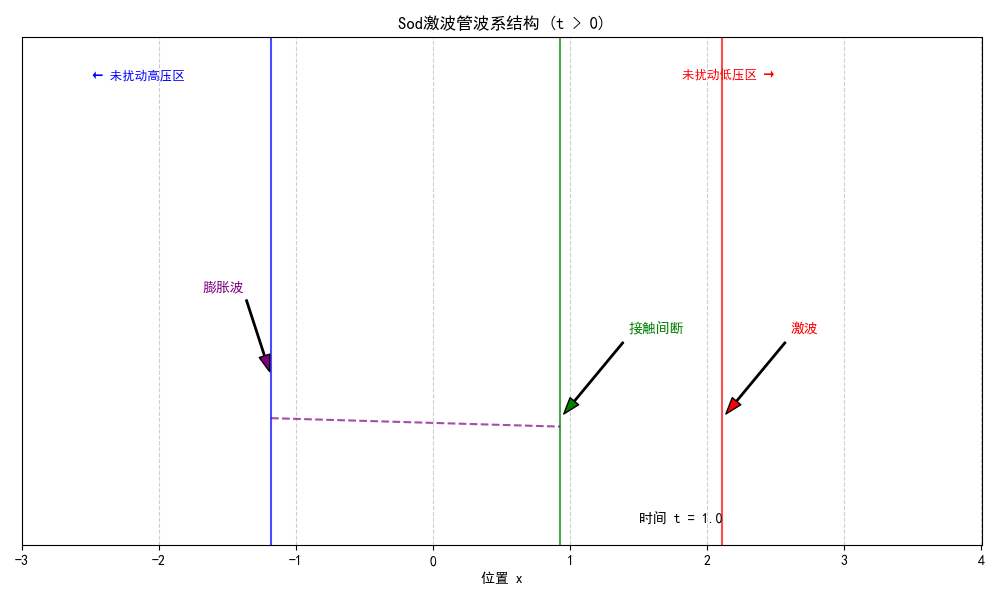
\includegraphics[width=0.8\textwidth]{wave_structure_1.png}
    \caption{Sod激波管典型波系结构(t>0)}
    \label{fig:wave_structure_1}
\end{figure}
\begin{figure}[H]
    \centering
    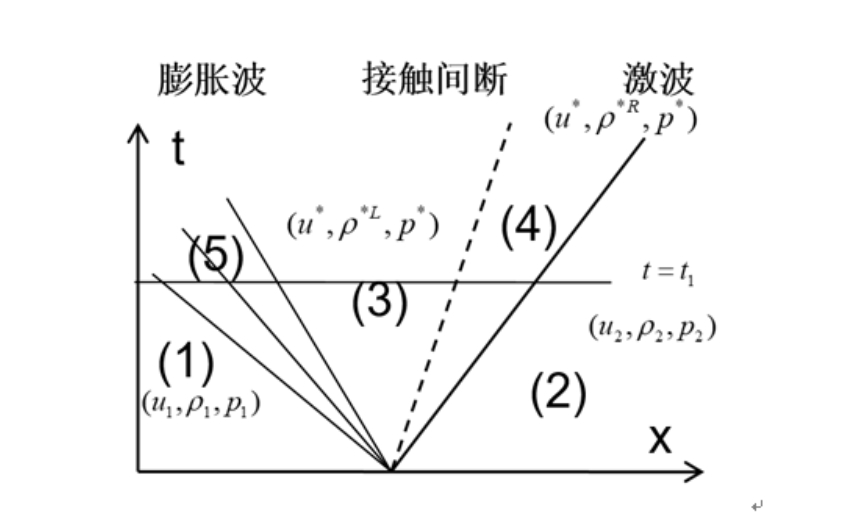
\includegraphics[width=0.8\textwidth]{wave_structure_2.png}
    \caption{Sod激波管典型波系结构}
    \label{fig:wave_structure_2}
\end{figure}
\subsubsection{解析解表达式}
解析解通过求解以下方程组获得:
\paragraph{1-3 两区, 等熵关系式}
$$\frac{p^{*}}{\left(\rho^{* L}\right)^{\gamma}}=\frac{p_{1}}{\left(\rho_{1}\right)^{\gamma}}$$
$$
u_{1}+\frac{2 c_{1}}{\gamma-1}=u^{*}+\frac{2 c^{L}}{\gamma-1}$$
其中, $c^{L}=\sqrt{\gamma p^{*} / \rho^{* L}}$。
\paragraph{2-4 两区, 激波 R-H 关系式}
$$\left\{\begin{array}{l}\rho_{2}\left(u_{2}-Z_{2}\right)=\rho^{* R}\left(u^{*}-Z_{2}\right) \\\rho_{2} u_{2}\left(u_{2}-Z_{2}\right)+p_{2}=\rho^{* R} u^{*}\left(u^{*}-Z_{2}\right)+p^{*} \\E_{2}\left(u_{2}-Z_{2}\right)+u_{2} p_{2}=E^{* R}\left(u^{*}-Z_{2}\right)+p^{*} u^{*}\end{array}\right.$$

以上变量说明从略。综上 5 个方程、 5 个未知数,故方程组可解,求解方法为联立以上两个方程组,解出 3、4 区内速度对压力的依赖关系,有

$$u^{*}=u_{1}-f(p^{*},p_{1},\rho_{1})$$

其中,满足 $$f(p^{*},p_{i},\rho_{i})=\frac{2c_{i}}{\gamma-1}\left[\left(\frac{p^{*}}{p_{i}}\right)^{\frac{\gamma-1}{2\gamma}}-1\right]$$。

注意到,激波、膨胀波前后速度-压力的依赖关系可写成统一的形式:

左波(激波或膨胀波)

$$u^{*}=u_{1}-f(p^{*},p_{1},\rho_{1})$$

右波(激波或膨胀波)

$$u^{*}=u_{2}+f(p^{*},p_{2},\rho_{2})$$

以上 $u^{*},p^{*}$ 表示 3、4 区内的速度与压力,其中

$$f(p^{*},p_{i},\rho_{i})=\left\{\begin{array}{ll}\frac{p^{*}-p_{i}}{\rho_{i}c_{i}\left[\frac{\gamma+1}{2\gamma}\left(\frac{p^{*}}{p_{i}}\right)+\frac{\gamma-1}{2\gamma}\right]^{1/2}}, & p^{*}>p_{i}\\\frac{2c_{i}}{\gamma-1}\left[\left(\frac{p^{*}}{p_{i}}\right)^{\frac{\gamma-1}{2\gamma}}-1\right], & p^{*}<p_{i}\end{array}\right.$$

求解上式可得到 3、4 区内的压力,然后可以解得速度和密度。
\paragraph{膨胀波内部}

对于膨胀波内部物理量的计算,首先由波头传播速度$u_1-c_1$与波尾传播速度$u^*-c^{*L}$
可计算膨胀波的范围。在膨胀波区内,利用特征相容关系和等熵关系计算物理量,可利
用简单波的特性来简化计算。以下直接给出各个物理量的计算表达式:
$$\begin{aligned}&c(t,x)=\frac{\gamma-1}{\gamma+1}\left(u_{1}-\frac{x}{t}\right)+\frac{2}{\gamma+1}c_{1}\\&u(x,t)=c+x/t\\&p=p_{1}\:(c/c_{1})^{2\gamma/\gamma-1}\\&\rho=\gamma p/c^{2}\end{aligned}$$
综上所述,一维 Riemann 问题的精确解的求解思路与方程介绍完毕。本文 Sod 激波管参考
精确解程序来自于 MATLAB 官方开源文档中的sod激波管的求解器 \cite{gogol2025}。

\subsection{数值计算方法}
% 补充边界条件说明
\subsubsection{计算域与网格}
针对 Sod激波管问题,选择对称计算域$[-L, L]$以满足激波传播的物理需求...网格收敛性分析需考察$N=100,200,400$等情形...

\textbf{边界条件设置:}
\begin{itemize}
    \item 计算域边界$x = \pm L$采用特征边界条件
    \item 边界值通过外推法处理: $U_0 = 2U_1 - U_2$, $U_{N+1} = 2U_N - U_{N-1}$
    \item 网格点$i=1$和$i=N$分别对应$x = -L + \Delta x / 2$和$x = L - \Delta x / 2$
\end{itemize}

% 修正minmod限制器和GVC格式
\subsubsection{激波捕捉格式}
1. TVD格式(Harten-Yee迎风格式):
$$\frac{\partial U_i}{\partial t} = -\frac{1}{\Delta x}\left(\hat{f}_{i+1/2} - \hat{f}_{i-1/2}\right)$$
数值通量构造:
$$\hat{f}_{i+1/2} = \frac{1}{2}\left[f(U_L) + f(U_R) - \Phi_{i+1/2}(U_R - U_L)\right]$$

\textbf{限制器函数:}
$$\Phi(r) = \text{minmod}(1, r) = 
\begin{cases} 
0 & \text{if } r \leq 0 \\
r & \text{if } 0 < r < 1 \\
1 & \text{if } r \geq 1 
\end{cases}, \quad r = \frac{U_i - U_{i-1}}{U_{i+1} - U_i}$$

2.群速度控制格式(GVC)修正:
$$\frac{\partial\hat{f}}{\partial x} \approx \frac{\hat{f}_{i+1/2} - \hat{f}_{i-1/2}}{\Delta x} + \tau\Delta x^2\frac{\partial^3 f}{\partial x^3}$$

\textbf{三阶导数项离散修正(迎风型):}
$$\left.\frac{\partial^3 f}{\partial x^3}\right|_i \approx 
\begin{cases}
\dfrac{2f_{i-3} - 9f_{i-2} + 18f_{i-1} - 11f_i}{\Delta x^3} & u \geq 0 \\
\dfrac{-11f_i + 18f_{i+1} - 9f_{i+2} + 2f_{i+3}}{\Delta x^3} & u < 0
\end{cases}$$
\textit{注: 根据局部流速方向选择迎风模板}


\subsubsection{数值通量计算方法}
\begin{enumerate}
    \item \textbf{通量向量分裂 (FVS - Steger-Warming格式)}  
    特征分裂处理对流项:
    $$f = f^+ + f^-,\quad f^\pm = A^\pm U$$
    其中$A^\pm = R\Lambda^\pm L$,特征值分解$\Lambda = \text{diag}(u,u+c,u-c)$,$\Lambda^\pm$取正负特征值部分。
    
    \item \textbf{通量差分分裂 (FDS - Roe格式)}  
    构造Roe平均矩阵$\tilde{A}_{i+1/2}$:
    \begin{align*}
    \tilde{\rho} &= \sqrt{\rho_L\rho_R},\quad \tilde{u} = \frac{\sqrt{\rho_L}u_L + \sqrt{\rho_R}u_R}{\sqrt{\rho_L} + \sqrt{\rho_R}} \\
    \tilde{H} &= \frac{\sqrt{\rho_L}H_L + \sqrt{\rho_R}H_R}{\sqrt{\rho_L} + \sqrt{\rho_R}},\quad \tilde{c} = \sqrt{(\gamma-1)\left(\tilde{H} - \frac{1}{2}\tilde{u}^2\right)}
    \end{align*}
    数值通量计算:
    $$\hat{f}_{i+1/2} = \frac{1}{2}\left[f(U_L)+f(U_R)\right] - \frac{1}{2}|\tilde{A}_{i+1/2}|(U_R - U_L)$$
\end{enumerate}

\subsubsection{时间推进方法}
采用三阶TVD Runge-Kutta方法离散时间项:
\begin{align*}
U^{(1)} &= U^n + \Delta t L(U^n) \\
U^{(2)} &= \frac{3}{4}U^n + \frac{1}{4}U^{(1)} + \frac{1}{4}\Delta t L(U^{(1)}) \\
U^{n+1} &= \frac{1}{3}U^n + \frac{2}{3}U^{(2)} + \frac{2}{3}\Delta t L(U^{(2)})
\end{align*}
其中$L(U)$为空间离散算子。时间步长由CFL条件约束:
$$\Delta t = \text{CFL}\cdot\frac{\Delta x}{\max(|u| + c)},\quad \text{CFL} \in [0.3, 0.6]$$
三阶精度与TVD特性保证激波捕捉的数值稳定性。



%附录
\newpage
\appendix
\section*{AI工具使用声明表}
\begin{table}[H]
    \centering
    \begin{tabular}{c|c|c}
        \hline
        使用内容 & 工具名称 & 使用目的 \\ \hline
        hw2.tex 1-9行、图片插入 & Github Copilot & 调整pdf格式,调用宏包,省略插入图片的重复性工作 \\ 
        main.py 6-15行 & DeepSeek & 修正 matplotlib 中文显示问题 \\ 
        ReadMe.md框架 & DeepSeek & 在DeepSeek的帮助下生成一个框架,在此基础上增加而来 \\
        .gitignore & Github Copilot & 针对于python和latex的.gitignore文件,完全由Copilot生成  
    \end{tabular}
    \label{tab:AI_tools}
\end{table}


\newpage
\section*{}
% 使用标准的BibTeX格式
\bibliographystyle{unsrturl} % 更改为支持URL的样式
\bibliography{reference} % 指定BibTeX数据库文件

\end{document}